\hypertarget{interfaceCqrs_1_1Akka_1_1Commands_1_1IConcurrentAkkaCommandPublisher}{}\section{Cqrs.\+Akka.\+Commands.\+I\+Concurrent\+Akka\+Command\+Publisher$<$ T\+Authentication\+Token, T\+Target $>$ Interface Template Reference}
\label{interfaceCqrs_1_1Akka_1_1Commands_1_1IConcurrentAkkaCommandPublisher}\index{Cqrs.\+Akka.\+Commands.\+I\+Concurrent\+Akka\+Command\+Publisher$<$ T\+Authentication\+Token, T\+Target $>$@{Cqrs.\+Akka.\+Commands.\+I\+Concurrent\+Akka\+Command\+Publisher$<$ T\+Authentication\+Token, T\+Target $>$}}


A I\+Akka\+Command\+Publisher$<$\+T\+Authentication\+Token$>$ that ensure concurrency regardless of what it passes the command onto as it is a Receive\+Actor  


Inheritance diagram for Cqrs.\+Akka.\+Commands.\+I\+Concurrent\+Akka\+Command\+Publisher$<$ T\+Authentication\+Token, T\+Target $>$\+:\begin{figure}[H]
\begin{center}
\leavevmode
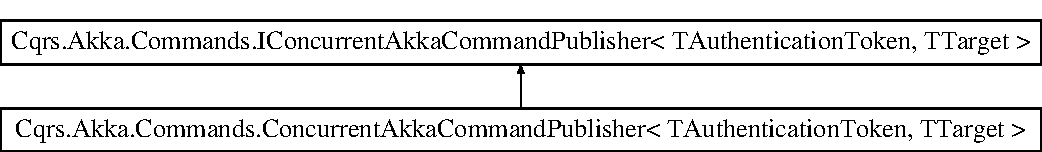
\includegraphics[height=2.000000cm]{interfaceCqrs_1_1Akka_1_1Commands_1_1IConcurrentAkkaCommandPublisher}
\end{center}
\end{figure}


\subsection{Detailed Description}
A I\+Akka\+Command\+Publisher$<$\+T\+Authentication\+Token$>$ that ensure concurrency regardless of what it passes the command onto as it is a Receive\+Actor 


\begin{DoxyTemplParams}{Template Parameters}
{\em T\+Authentication\+Token} & The Type of the authentication token.\\
\hline
{\em T\+Target} & The Type of the object that is targeted that needs concurrency.\\
\hline
\end{DoxyTemplParams}
